\chapter*{First Steps in New System}
\section*{Getting Oriented}

You're now looking at the GNOME Shell environment. The first thing you'll probably notice when you start working with GNOME Shell for the first time is that application windows only have the \emph{Close} button. The GNOME desktop environment tries to be as simple as possible and because you can maximize windows by dragging them to the top of the screen, minimize them by dragging them away from the top of the screen, or do both by double clicking the title bar, there is no need to have dedicated \emph{Minimize} and \emph{Maximize} buttons.

\begin{figure}[ht]
\begin{center}
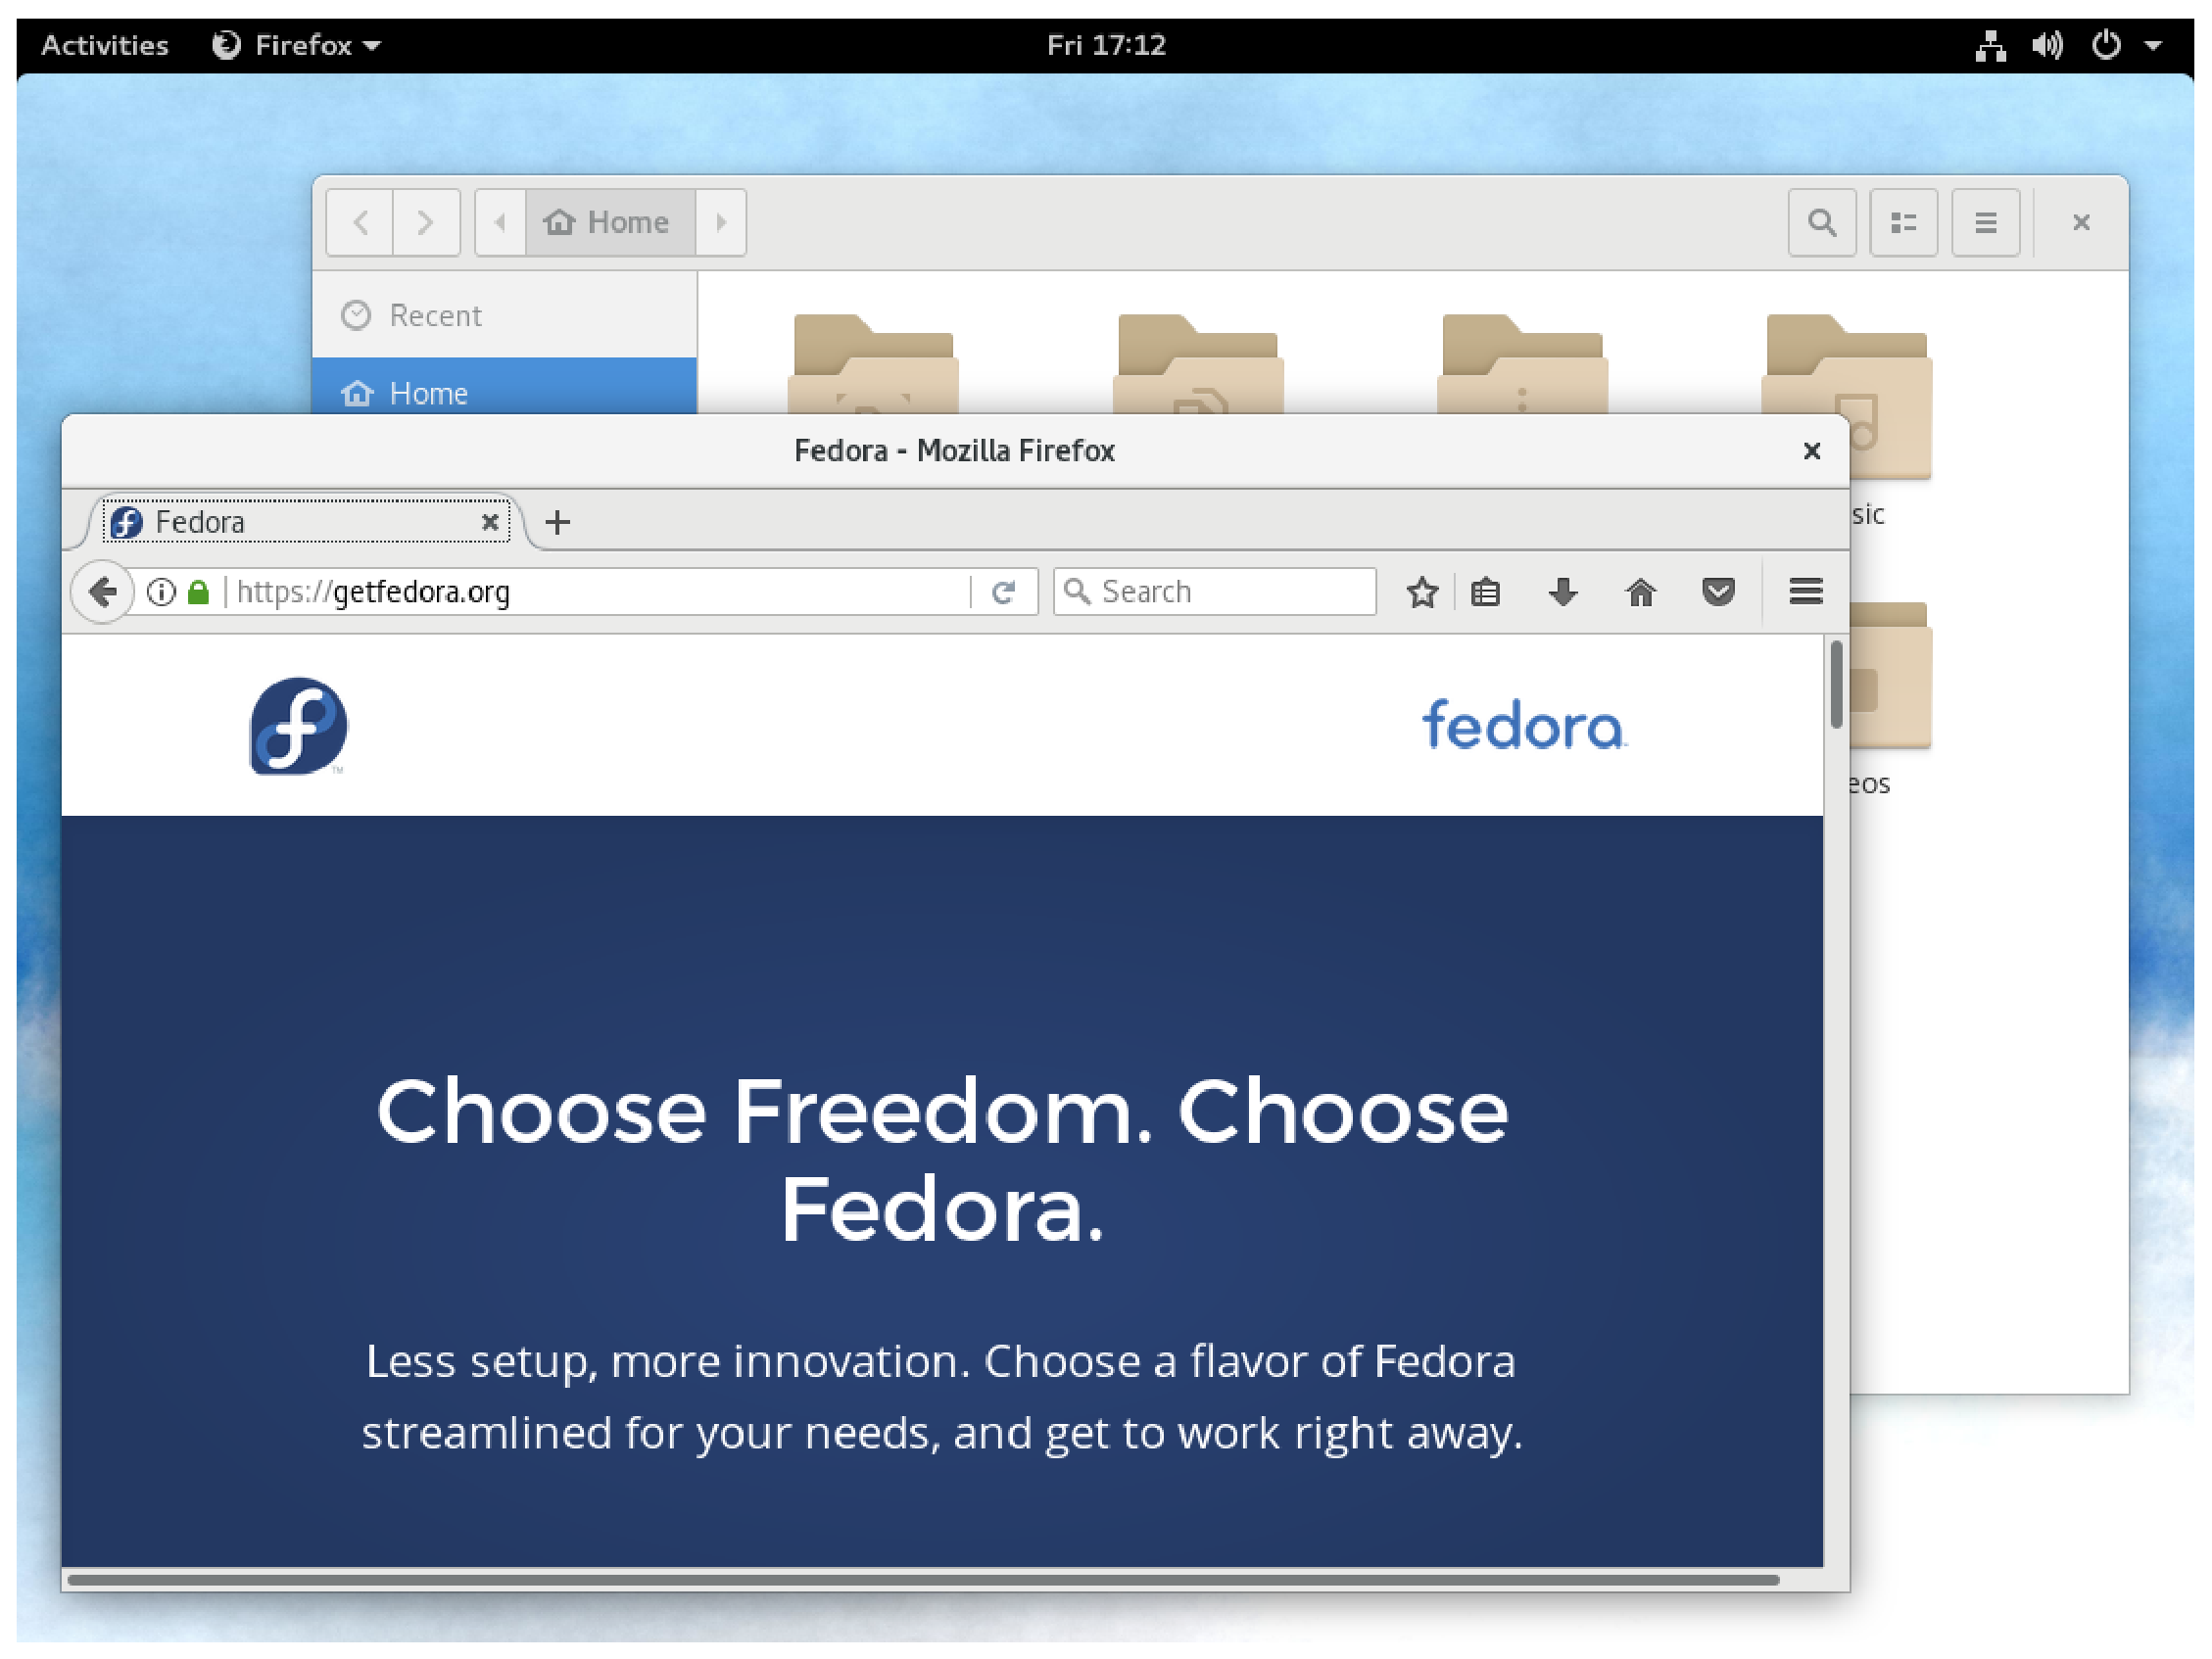
\includegraphics[width=0.95\textwidth]{img/shell-a}
\captionbelow{The initial screen of GNOME Shell} \label{fig:shell-a}
\end{center}
\end{figure}

The top part of the screen includes the following items:
\begin{enumerate}
\item The \emph{Activities} button -- this button gives you access to the \emph{Activities Overview} and is the starting point for the majority of activities you typically expect from a desktop installation. We'll be taking a closer look at it in the next section.

\item The \emph{Application Menu} -- clicking the name of the active application in the top left corner of the screen gives you access to the options that are relevant for the application as a whole: typically, you will find menu entries like \emph{Preferences}, \emph{About}, and \emph{Help} here. Options that are only relevant for individual windows are typically accessible from the windows themselves. Not all applications utilize the \emph{Application Menu} and will only have the \emph{Quit} option in it.

\begin{figure}[ht]
\begin{center}
\includegraphics[width=0.45\textwidth]{img/app-menu}
\captionbelow{The Application Menu} \label{fig:app-menu}
\end{center}
\end{figure}

\item The \emph{Clock and Calendar} applet -- clicking the current time in the top middle part of the screen gives you access to a list of missed notifications and also a calendar. If you use one of the applications that use the calendar back end of GNOME (such as \emph{Evolution}), you'll also see events you entered in those applications.

\begin{figure}[ht]
\begin{center}
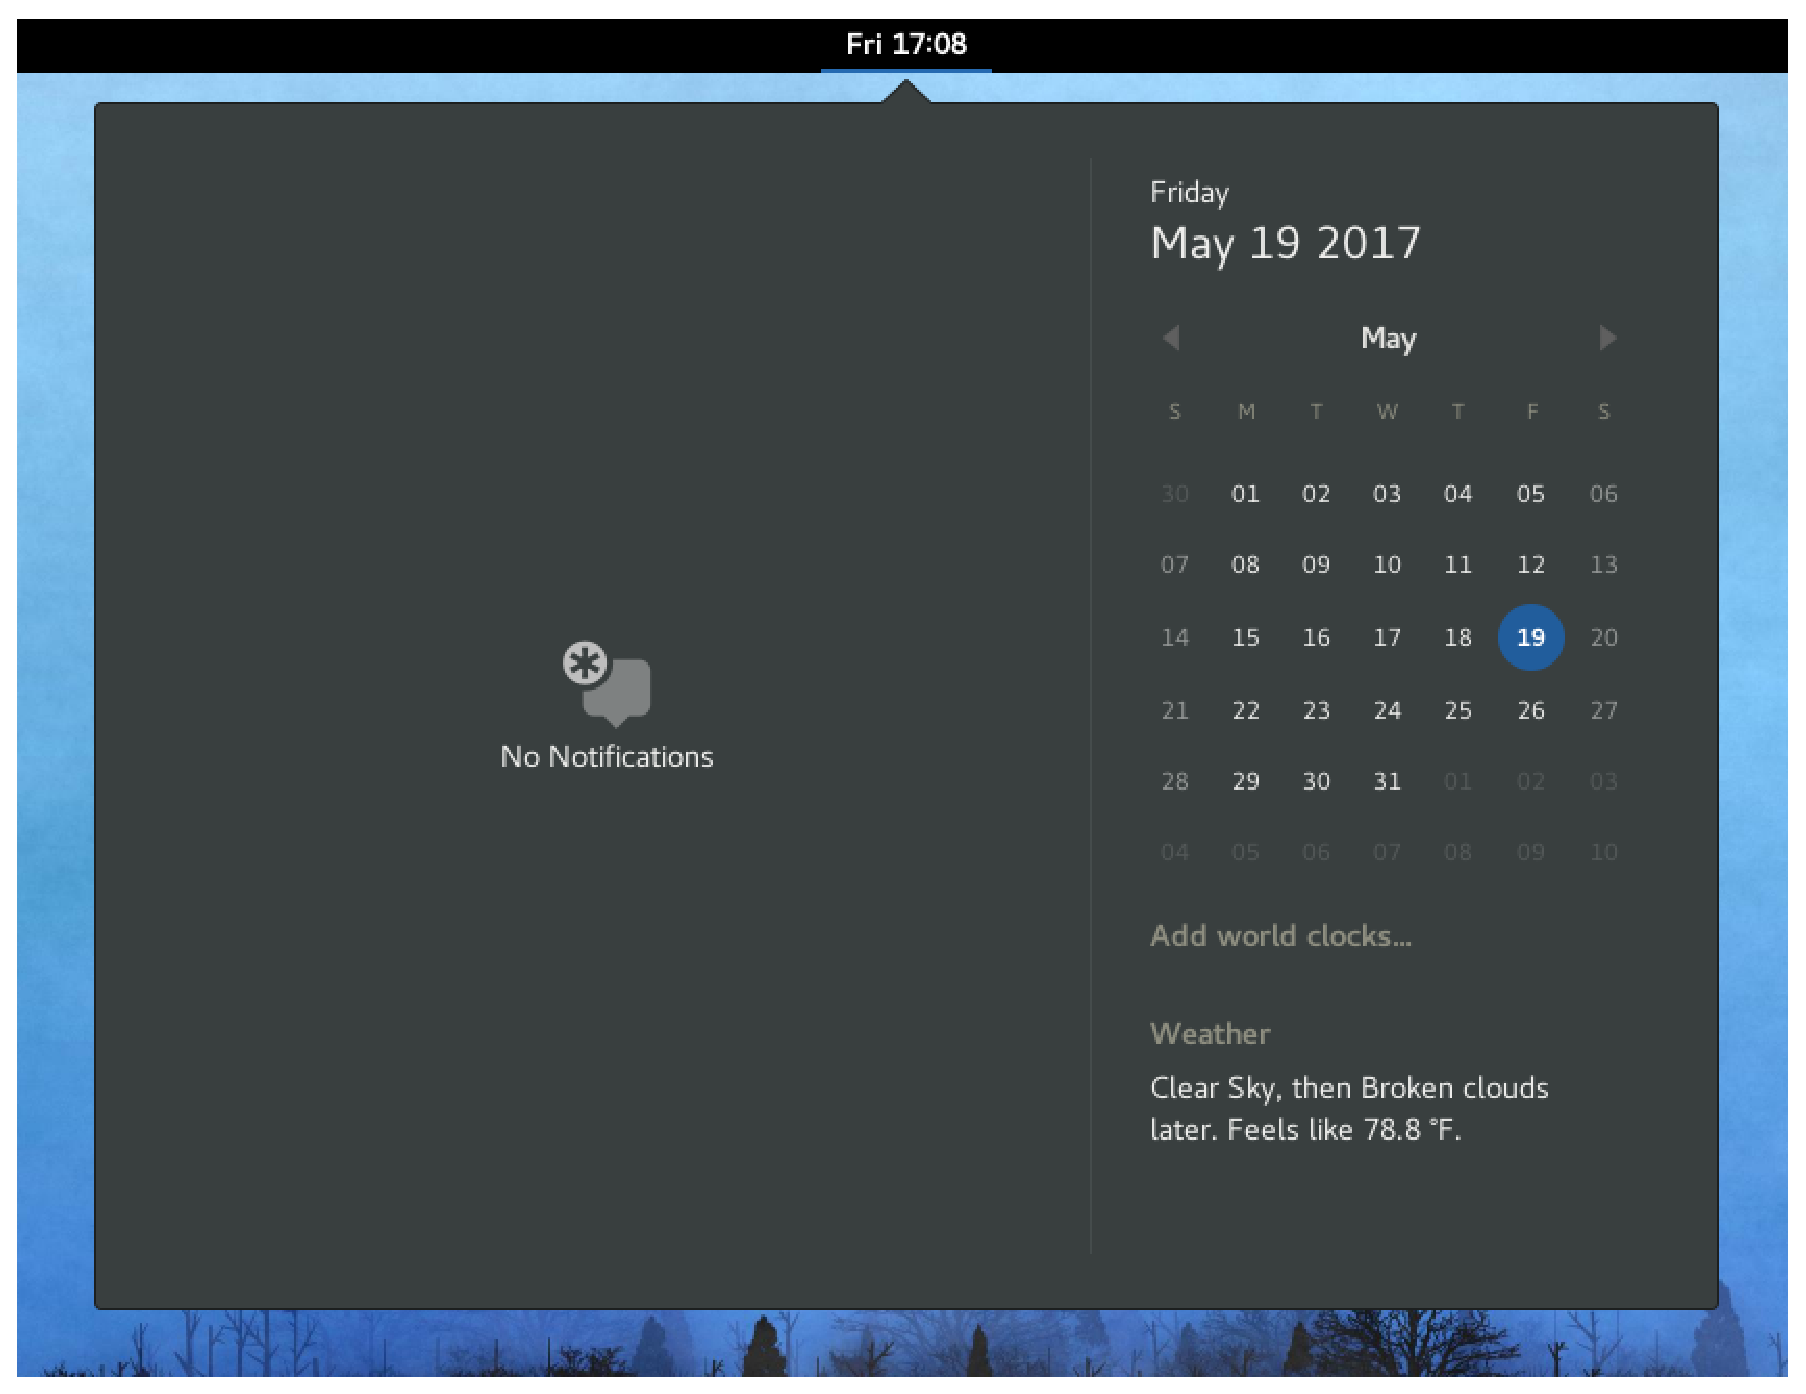
\includegraphics[width=0.75\textwidth]{img/calendar}
\captionbelow{The Clock and Calendar applet} \label{fig:calendar}
\end{center}
\end{figure}

\item The \emph{User Menu} -- in the upper right corner of the screen are located the most important indicators: the network connection status, the volume icon, and the battery status. Clicking on either of them will open a menu that will allow you to adjust the volume, change the brightness of your screen, select a suitable network connection option, connect to Bluetooth devices, and so on. Clicking on your name in this menu will give you an option to log out of the current session or switch to a different account. Finally, at the very bottom of this menu, you'll find three buttons: the left button will open the system settings, the middle button will lock the screen, and the right button will give you the option to restart or power off your machine.
\end{enumerate}

\begin{figure}[ht]
\begin{center}
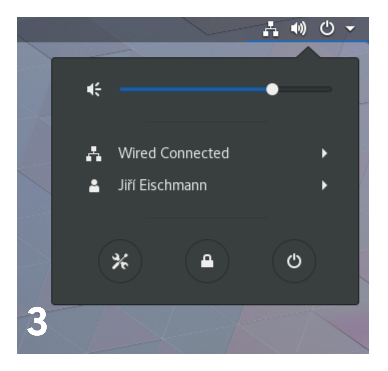
\includegraphics[width=0.45\textwidth]{img/menu}
\captionbelow{The User Menu} \label{fig:menu}
\end{center}
\end{figure}

\section*{Exploring the Activities Overview}

The key part of the user interface is the \emph{Activities} button located in the upper left corner of the screen. You don't even need to click it, just move the mouse pointer to the upper left corner or press the \keystroke{Super} key (also known as the \keystroke{Windows} key). When you do so, you will be presented with the \emph{Activities Overview} that will show you all currently open windows, give you access to installed applications, and allow you to switch between virtual workspaces.

\begin{figure}[ht]
\begin{center}
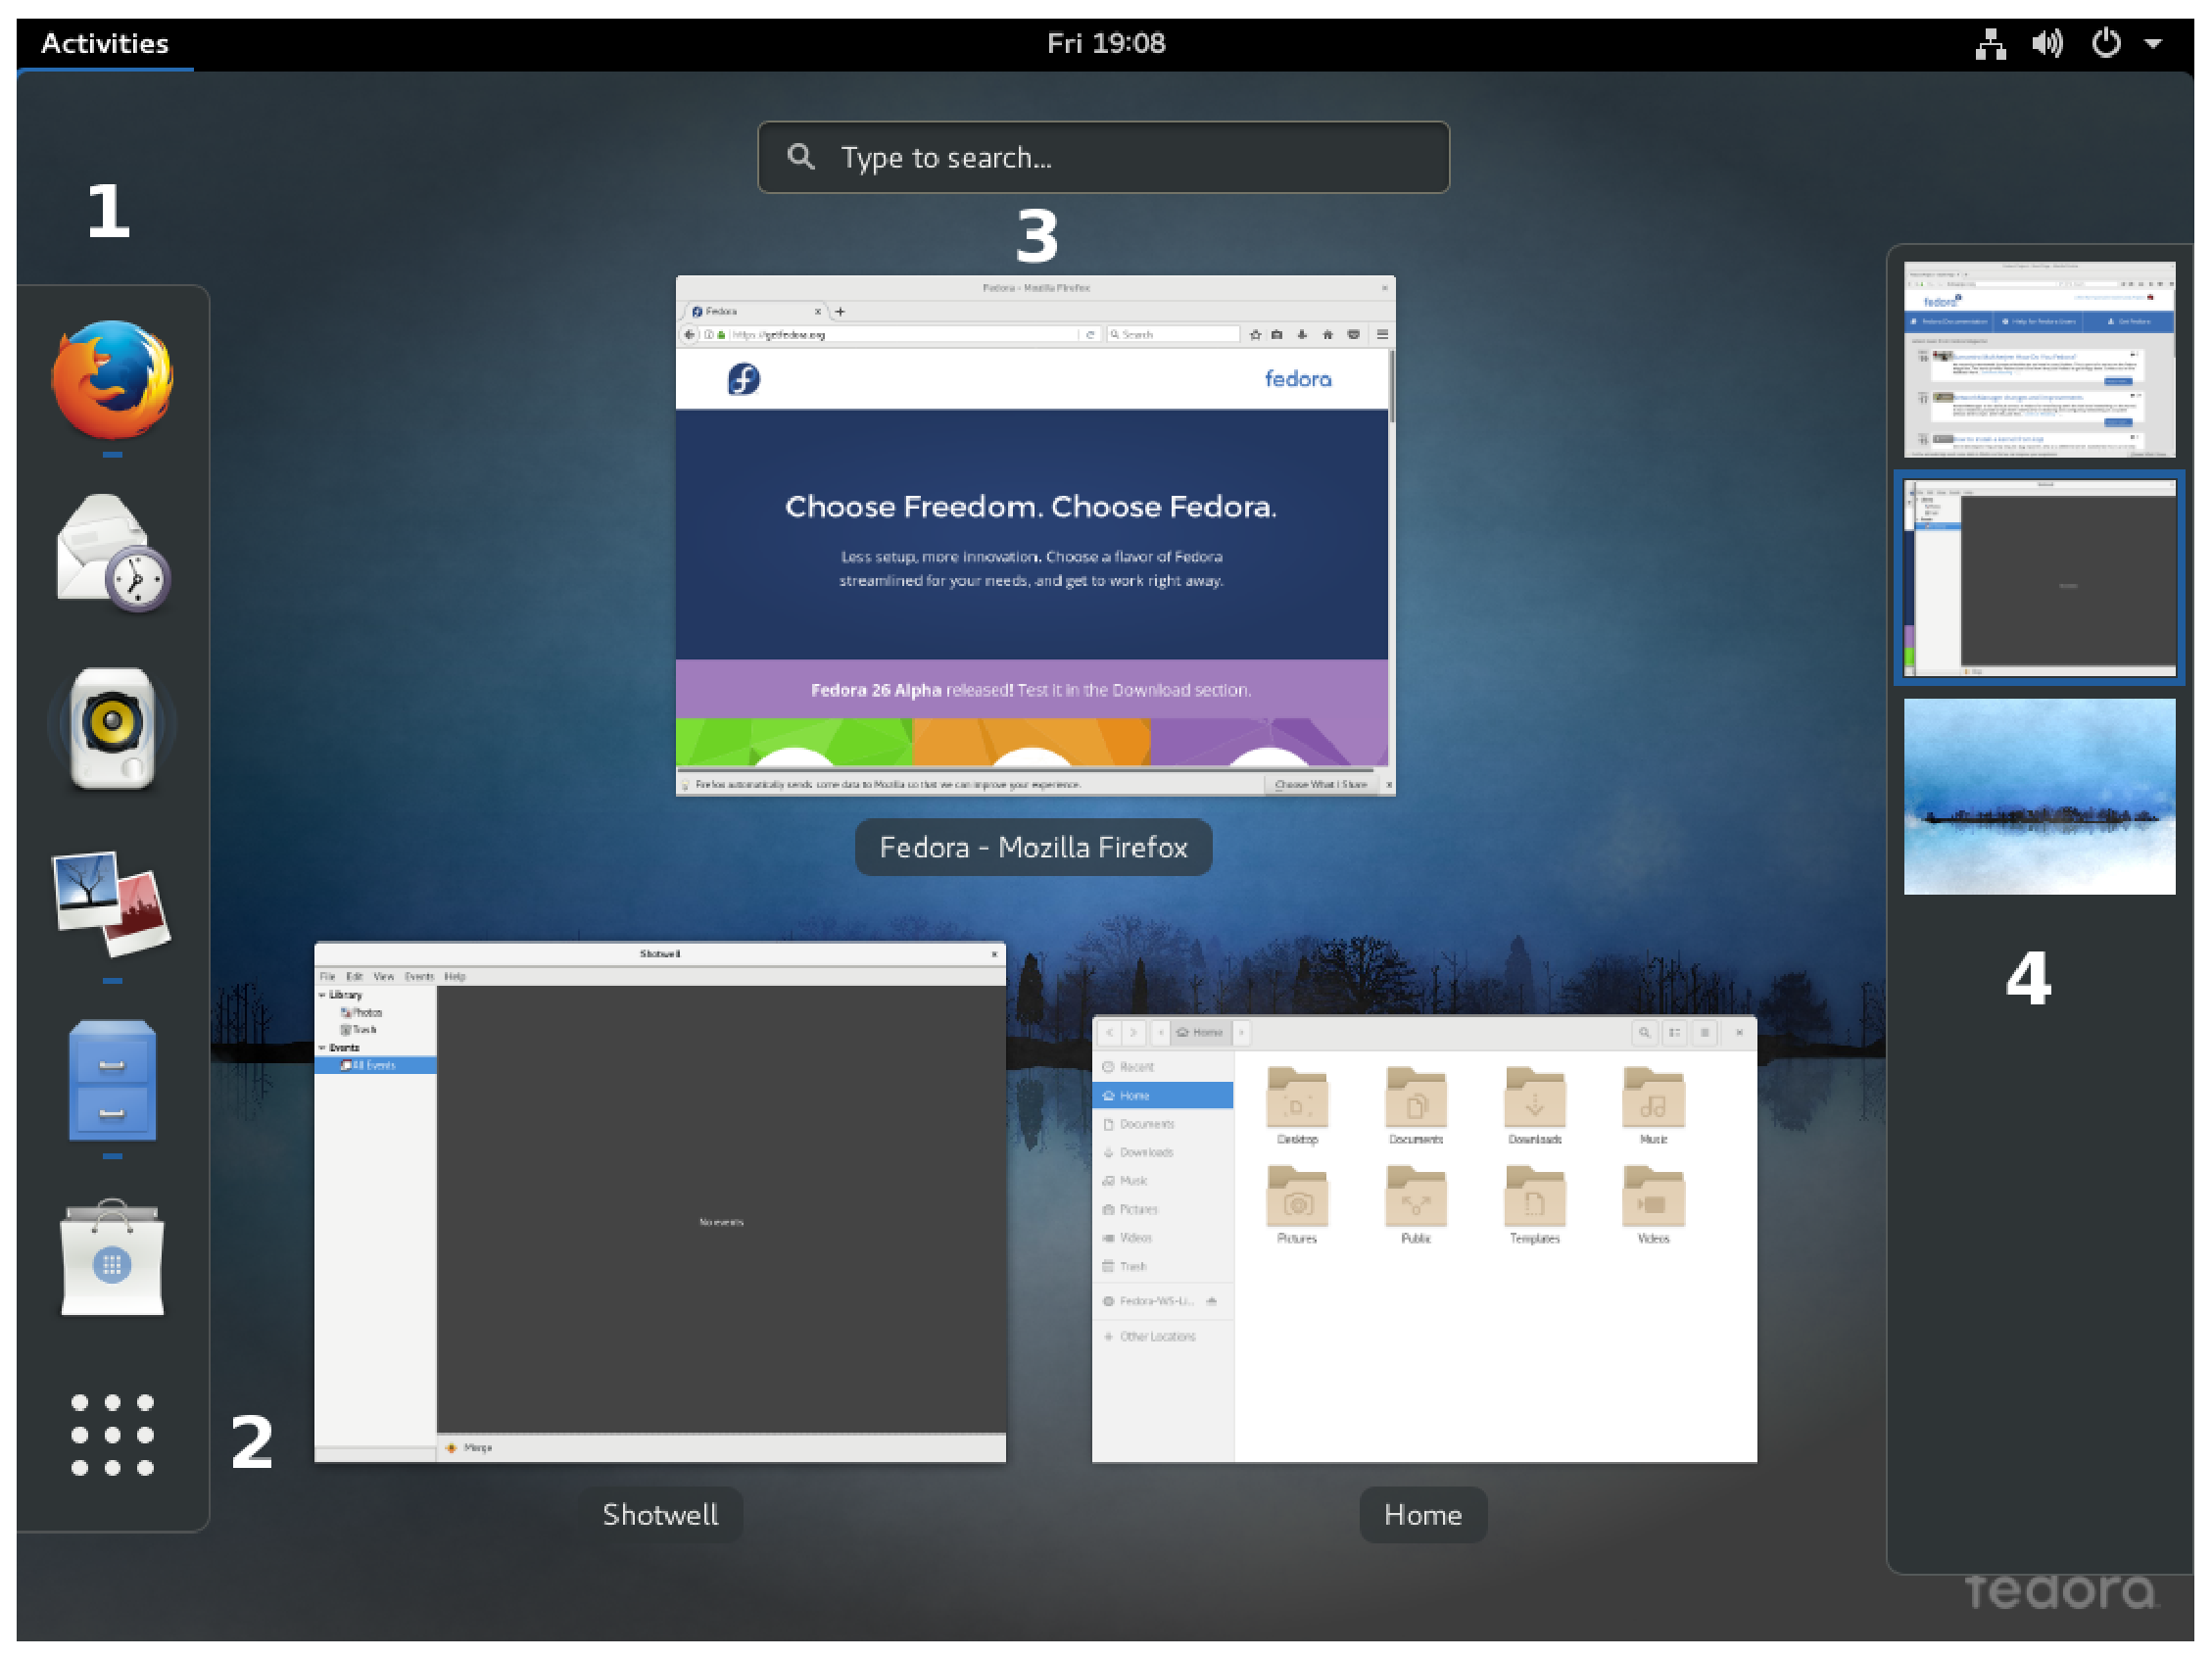
\includegraphics[width=0.95\textwidth]{img/shell-b}
\captionbelow{The Activities Overview} \label{fig:shell-b}
\end{center}
\end{figure}

The \emph{Activities Overview} consists of the following key components:
\begin{enumerate}
\item The \emph{Dash} -- the vertical panel along the left side of the screen gives you a quick access to all currently running applications and to those that you've marked as your favorite ones. Running applications are clearly underlined. If you want to mark a running application as your favorite, click its icon with the right mouse button and select \emph{Add to Favorites} from the menu.

\begin{figure}[ht]
\begin{center}
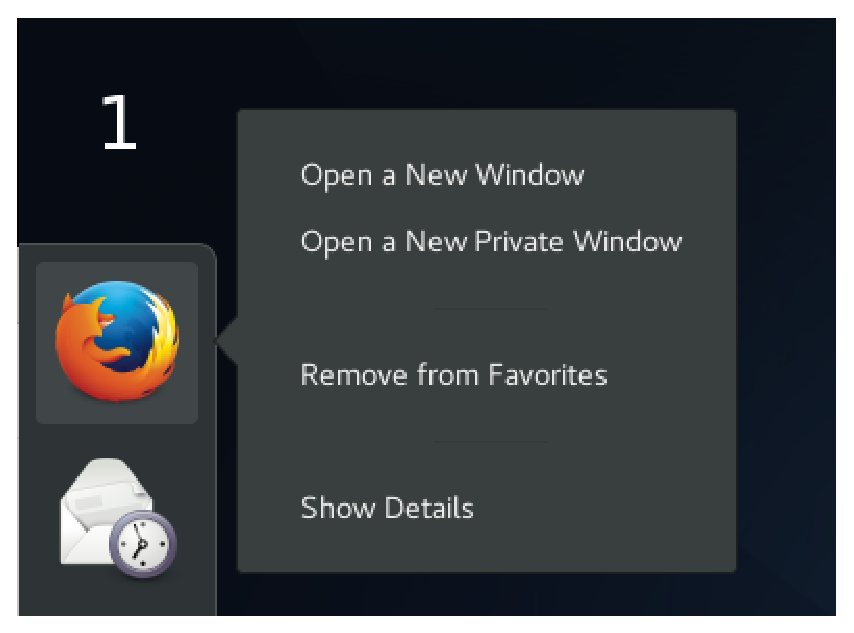
\includegraphics[width=0.45\textwidth]{img/dash-b}
\captionbelow{Working with applications in Dash} \label{fig:dash-b}
\end{center}
\end{figure}

\item The \emph{Show Applications} button -- at the bottom of the \emph{Dash}, you can find an icon depicting a grid of squares that says "Show Applications" when you move the mouse pointer over it. Click on it to get a list of application launchers. You can switch between launchers for frequently used applications and launchers for all installed applications by clicking the respective buttons at the bottom of the screen.

\begin{figure}[ht]
\begin{center}

\includegraphics[width=0.45\textwidth]{img/dash-a}
\captionbelow{The Show Applications button} \label{fig:dash-a}
\end{center}
\end{figure}

\item The \emph{Search} field -- if you know the name of the application you're looking for or at least a part of it, after opening the \emph{Activities Overview}, you can just start typing the name and you don't even need to select the search field at the top of the screen. As you type, GNOME Shell will not only show you all matching applications, but it will also offer you matching contacts, documents, pictures, settings, and so on. You can change what you want to include in the search results in the System Settings under \emph{Search}.

Using the \emph{Search} field is probably the fastest way to launch applications in GNOME.

\begin{figure}[ht]
\begin{center}
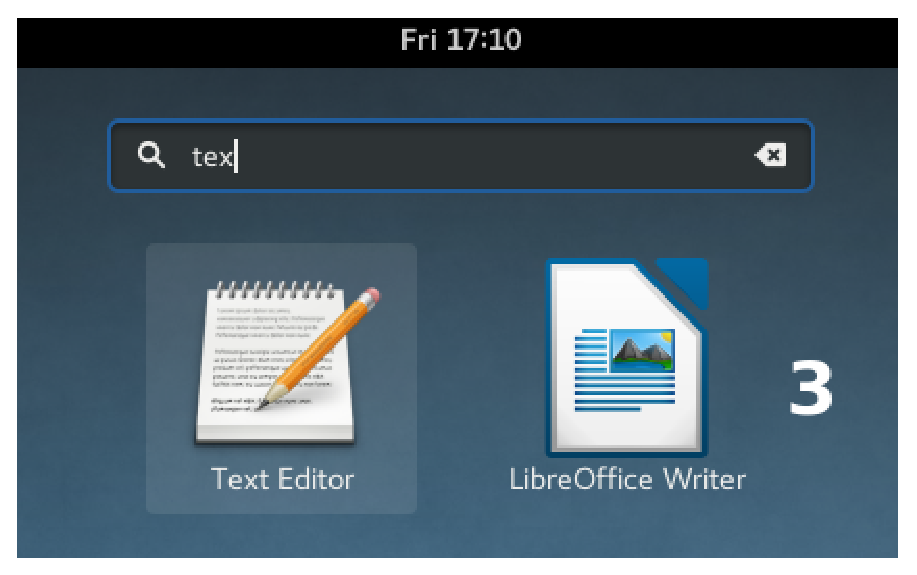
\includegraphics[width=0.85\textwidth]{img/search}
\captionbelow{Using the Search field} \label{fig:search}
\end{center}
\end{figure}

\item \emph{Virtual Workspaces} -- the vertical panel along the right side of the screen gives you an overview of your virtual workspaces. Virtual workspaces provide you with a convenient way to organize application windows rather than having all of them on a single screen. In GNOME, you don't have a fixed number of workspaces available to you, but as many as you need. Whenever you drag an application window to an empty workspace, GNOME automatically adds a new empty one below it for you. It also automatically deletes surplus empty workspaces to make sure there is always exactly one without any windows in it.

You can use keybord shortcuts to move between virtual workspaces. Press $\keystroke{Ctrl}+\keystroke{Alt}+\keystroke{arrow $\uparrow$}$ to switch to the workspace directly above the current one, or $\keystroke{Ctrl}+\keystroke{Alt}+\keystroke{arrow $\downarrow$}$ to switch to the workspace directly below the one you are on.

\item The \emph{Preview of Open Windows} -- the middle part of the screen is used to give you an overview of all open windows. You can switch to a particular window by clicking on it with the left mouse button. If you prefer to use your keyboard, after entering the \emph{Activities Overview}, press \keystroke{arrow $\downarrow$} and then use arrow keys to navigate between the windows. Press \keystroke{Enter} to switch to the selected window.

\section*{Adjusting System Settings}

To change system and user settings, open the \emph{All Settings} window either by selecting \emph{Settings} from the list of application launchers, or by typing "Settings" in the \emph{Search} field as described above.


\begin{figure}[p]
\begin{center}
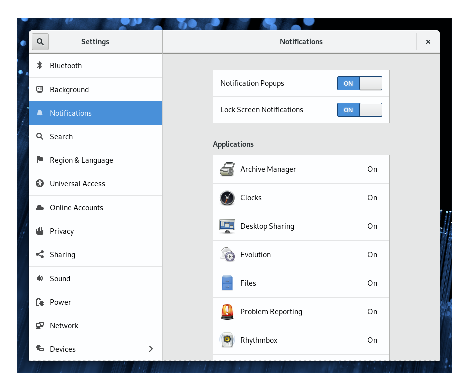
\includegraphics[width=0.72\textwidth]{img/settings}
\captionbelow{User and system settings} \label{fig:settings}
%\end{center}
%\end{figure}
\bigskip
%\begin{figure}[t]
%\begin{center}
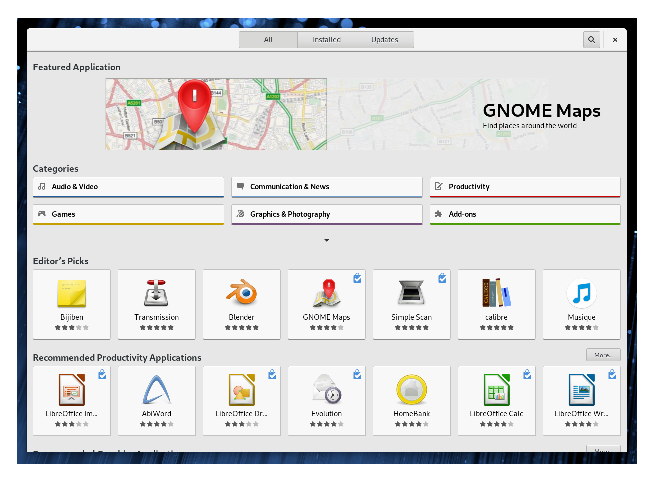
\includegraphics[width=0.72\textwidth]{img/software}
\captionbelow{Software management in Fedora} \label{fig:software}
\end{center}
\end{figure}

In GNOME, settings are split into three categories: \emph{Personal}, \emph{Hardware}, and \emph{System}. Here you can configure anything from the desktop background and the system language to printers, network connections, and user accounts. You can also connect to different online accounts in cloud services such as Nextcloud, Google, and Facebook and allow different desktop applications to access your data stored in those services. Do you use instant messaging and need to access your contacts? This way you will only need to log in to your cloud account once and all your contacts will be immediately accessible.
\end{enumerate}

\section*{Installing Additional Software}

Fedora Workstation includes a lot of commonly used applications in the default installation: \emph{Mozilla~Firefox} as the default web browser, \emph{LibreOffice} as the office suite, \emph{Totem} as a multimedia player, and many more. But what if you need something else?

Of course, not all software can be included in the default installation. Thousands of software packages are therefore readily available in so called "repositories" from which you can easily download them. Repositories are hosted on remote servers and their mirrors and provide packages of different applications and libraries. Have you heard of \emph{app stores} on mobile platforms? The basic principal is the same. If you want to download and install a program from the web, first check if it is not already available in the repositories. That's how you install most applications on Linux.

So how do you install additional software? Basically, you have two options:
\begin{enumerate}
\item Use the graphical application called \emph{Software} -- \emph{Software} offers exactly what you would expect from similar applications on mobile platforms: it is an elegant and easy-to-use gateway to repositories that allows you to search for applications and their add-ons, or browse applications from different categories. Each application has its own profile with a brief description, license, size information, and so on. And of course, all applications are open source and free to use.

In addition, \emph{Software} allows you to uninstall applications you no longer want on your system. You can also use it to update the system and installed packages.

%.Software management in Fedora
%image::img/software.png[width=500]

\item Use \emph{dnf} on the command line or its graphical interface -- \emph{Software} allows you to search for and install desktop applications from the repositories, but will not offer you other types of packages, such as libraries, command-line tools, or documentation. Nevertheless, the Fedora repositories host almost 20,000 packages and most of them don't represent desktop applications. To find, install, uninstall, or update such packages, use the command-line tool called \emph{dnf} or its graphical interface called \emph{Yum extender (DNF)}, which will give you the comfort of desktop applications.
\end{enumerate}

\section*{Codecs and Other Software}

What if some software is not available in the Fedora repositories? This can happen, you may need a specific codec or a driver that can be distributed free of charge, but for various reasons (typically because of its license or patents) it can't be distributed by the Fedora Project. That's where third-party repositories may come in handy.

Third-party repositories are not maintained by the Fedora Project and are not associated with it in any way. It's important to note that the Fedora Project is not liable for those software sources and cannot even guarantee that they will be in accordance with your local copyright and patent laws.

Typically, you will find three types of third-party repositories:
\begin{enumerate}
\item\emph{Vendor repositories} -- corporations such as Google or Adobe offer software sources that include their products, from development utilities to programs such as \emph{Google Chrome} and the \emph{Adobe Flash Player} plugin. A package installed from their website usually enables their repository in order to receive future updates. Once a repository is added to the software sources, you will be able to find the packages it provides by using already mentioned tools, \emph{Software} and \emph{dnf}. You can manage those packages like any other packages available from the official Fedora repositories.

\item\emph{Other repositories} -- there are several large third-party software sources with many packages that usually include software that is not open source or is patent-protected. For example, you may find multimedia codecs or specific drivers in repositories such as \emph{RPMFusion}. After you add the repositories, you install packages from them the same way you would install them from the official Fedora repositories.

\item\emph{Copr repositories} -- unlike in the previous cases, software in Copr repositories has always its license compatible with Fedora. Copr repositories are easy to add and are the biggest source of software for Fedora outside of the official repositories. They include the newest, often development versions of desktop environments, applications, and frameworks and you can find them at \url{copr.fedoraproject.org}.
\end{enumerate}

Before installing any packages from third-party repositories, make sure that you understand what they change in your system. You should not blindly install software that is not officially shipped by the Fedora Project and should always check if the source can be trusted and packages it provides won't do any harm to your system.

\endinput
